\myheading{Gaussian elimination: Kirchhoff’s circuit laws}

\renewcommand{\CURPATH}{linear/gauss}

\leveldown{}

The circuit I've created on
falstad.com\footnote{\url{http://falstad.com/circuit/}}:

\begin{figure}[H]
\centering
\frame{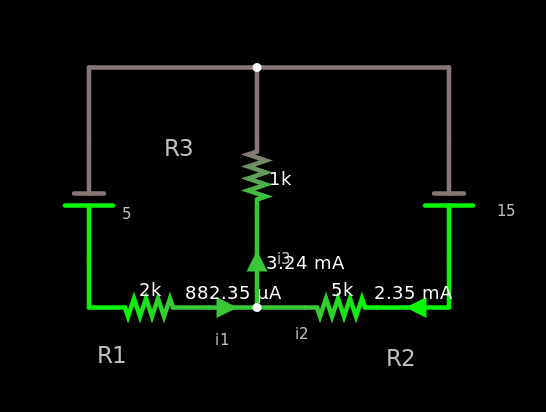
\includegraphics[scale=0.7]{\CURPATH/kirk.png}}
\end{figure}

Click here to open it on their website and run: \url{http://tinyurl.com/y8raoud3}.

The problem: find all 3 current values in 2 loops.
This is usually solved by solving a system of linear equations.

Overkill, but Z3 SMT-solver can be used here as well, since it can solve linear equations as well, over real numbers:

\lstinputlisting[style=custompy]{\CURPATH/kirk.py}

And the result:

\begin{lstlisting}
sat
[i3 = 11/3400, i1 = 3/3400, i2 = 1/425]
0.000882?
0.002352?
0.003235?
\end{lstlisting}

Same as on falstad.com online simulator.

Z3 represents real numbers as fractions, then we convert them to numerical form...

Further work: take a circuit as a graph and build a system of equations.

\myheading{Gaussian elimination}

SMT-solver is overkill, these linear equations can be solved using simple and well-known Gaussian elimination.

First, we rewrite the system of equation:

\begin{lstlisting}
   i1 +    i2 -    i3 == 0
R1*i1 +         R3*i3 == V1
        R2*i2 + R3*i3 == V2
\end{lstlisting}

Or in matrix form:

\begin{lstlisting}
[ 1,    1,    -1    | 0  ]
[ 2000, 0,    1000  | 5  ]
[ 0,    5000, 1000  | 15 ]
\end{lstlisting}

I can solve it using Wolfram Mathematica, using RowReduce
\footnote{\url{http://reference.wolfram.com/language/ref/RowReduce.html}}.

\begin{lstlisting}
In[1]:= RowReduce[{{1, 1, -1, 0}, {2000, 0, 1000, 5}, {0, 5000, 1000, 15}}]
Out[1]= {{1,0,0,3/3400},{0,1,0,1/425},{0,0,1,11/3400}}

In[2]:= 3/3400//N
Out[2]= 0.000882353

In[3]:= 1/425//N
Out[3]= 0.00235294

In[4]:= 11/3400//N
Out[4]= 0.00323529
\end{lstlisting}

This is the same result: i1, i2 and i3 in numerical form.

ReduceRow's output is:

\begin{lstlisting}
[ 1,0,0 | 3/3400  ]
[ 0,1,0 | 1/425   ]
[ 0,0,1 | 11/3400 ]
\end{lstlisting}

... back to expressions, this is:

\begin{lstlisting}
1*i1 + 0*i2 + 0*i3 = 3/3400
0*i1 + 1*i2 + 0*i3 = 1/425
0*i1 + 0*i2 + 1*i3 = 11/3400
\end{lstlisting}

In other words, this is just what i1/i2/i3 are.

Now something down-to-earth, C example I've copypasted from 
Rosetta Code
\footnote{\url{https://rosettacode.org/wiki/Gaussian_elimination\#C}},
working with no additional libraries, etc:

\lstinputlisting[style=customc]{\CURPATH/g.c}

I run it:

\begin{lstlisting}
0.000882353
0.00235294
0.00323529
\end{lstlisting}

See also: \url{https://en.wikipedia.org/wiki/Gaussian_elimination}, \\
\url{http://mathworld.wolfram.com/GaussianElimination.html}.

But a fun with SMT solver is that we can solve these equations without any knowledge of linear algebra, matrices,
Gaussian elimination and whatnot.

According to the source code of Z3, it can perform Gaussian Elimination, perhaps, whenever it can do so.

Some people try to use Z3 to solve problems with operational amplifiers:
\href{https://stackoverflow.com/questions/16552770/how-to-use-z3py-online-to-solve-problems-with-operational-amplifiers}{1},
\href{https://stackoverflow.com/questions/19317677/how-to-use-z3-smt-lib-online-to-solve-problems-with-operational-amplifiers}{2}.

\levelup{}

